\chapter{Zrealizowany system wizyjny do detekcji ludzi} %OK TODO 2 napisać do czego...
\label{cha:propSysWiz}

\begin{figure}
\centering
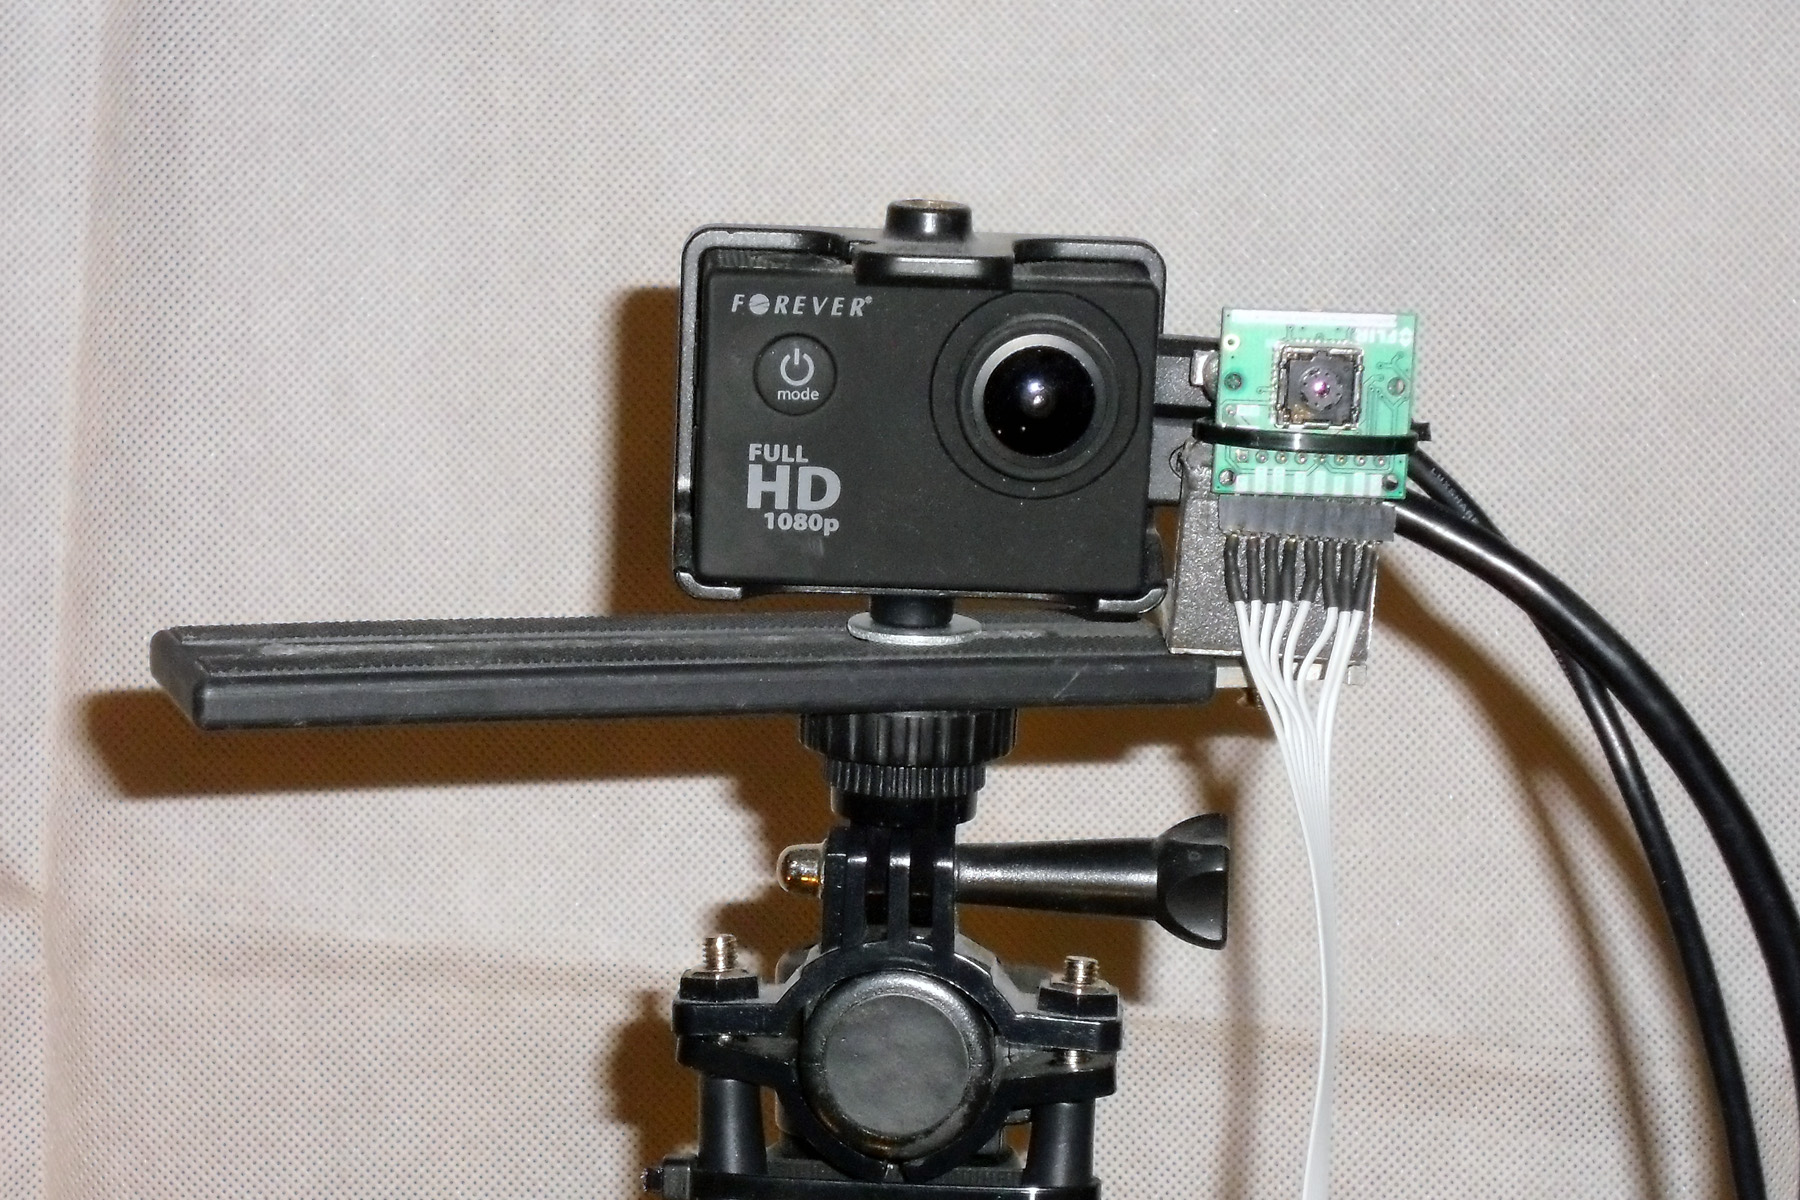
\includegraphics[width=0.65\linewidth]{images/kameraRGBIR.jpg}
\caption[Wykorzystany system kamer.]{Wykorzystany system kamer. Po lewej stronie znajduje się kamera wizyjna, po prawej termowizyjna Lepton.}
\label{fig:kameraRGBIR}
\end{figure}

\begin{figure}
\centering
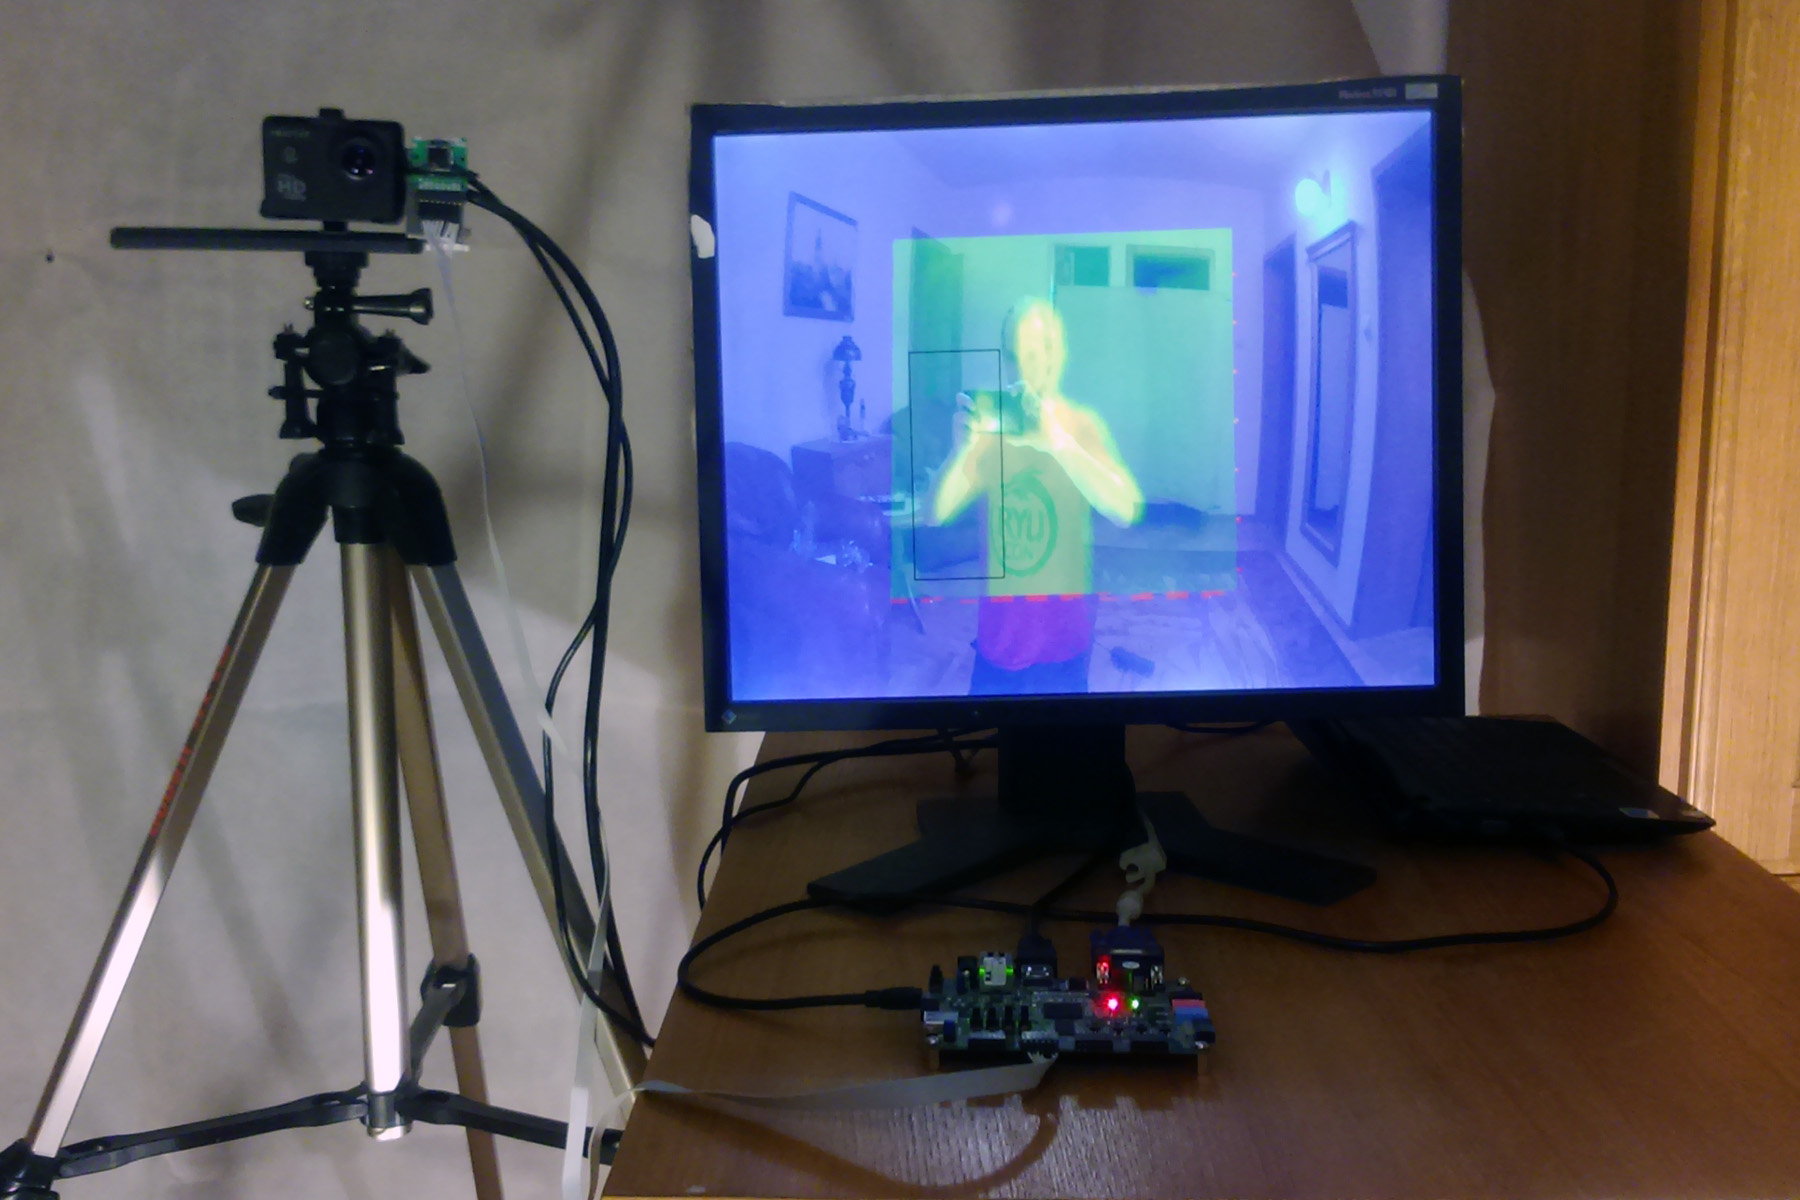
\includegraphics[width=0.65\linewidth]{images/systemOverview.jpg}
\caption[Widok na kompletny system.]{Widok na kompletny system do detekcji obiektów w przestrzeni multispektralnej. Obraz jest rejestrowany przez zespół kamer znajdujący się na statywie. Kamery są połączone do płytki deweloperskiej Zybo. Wynik jest prezentowany na monitorze.}
\label{fig:systemOverview}
\end{figure}

\section{Koncepcja systemu}

Zadaniem systemu jest detekcja osób na obrazie multispektralnym. 
Do uzyskania obrazu multispektralnego została wykorzystana kamera wizyjna, dająca obraz o~rozdzielczości 640x480 pikseli i~50 klatek na sekundę oraz termowizyjna: Lepton -- 80x60 pikseli i~9 klatek na sekundę. 
Obraz z~kamery termowizyjnej (IR) jest dopasowywany do wizyjnego (RGB) za pomocą projekcji perspektywicznej. 
Wynikiem ich połączenia jest obraz multispektralny (RGBIR). 
Wybór ROI odbywa się tylko z wykorzystaniem obrazu termowizyjnego. 
W~tym celu został wykorzystany moduł PDM (ang. \textit{Probability Density Matrix}) zaczerpnięty z pracy inżynierskiej autora \cite{kankaing}.
Tworzy on listę kandydatów, z której jest wybierany najbardziej prawdopodobny wynik. 
Następnie z ROI o wymiarach 80x192 piksele wyodrębniane są deskryptory HOG oraz przeprowadzana jest klasyfikacja z wykorzystaniem SVM. 
Wynik detekcji jest prezentowany na ekranie, poprzez obramowanie sylwetki przechodnia.
Do realizacji tego systemu została wykorzystana płytka deweloperska ZYBO firmy Digilent. 
Bazuje ona na omówionym wcześniej w~rozdziale \ref{cha:fpga} układzie Zynq-7000. 
Jest to układ heterogeniczny, co daje możliwość realizacji poszczególnych elementów systemu wizyjnego w~logice programowalnej (PL) lub systemie procesorowym (PS)
Zaproponowano następujący podział zadań:

Logika programowalna:
\begin{itemize}
\item Akwizycja obrazu poprzez HDMI (RGB) i VoSPI (IR),
\item Transformata projekcyjna i interpolacja obrazu IR,
\item Nałożenie i synchronizacja obrazu IR do obrazu RGB,
\item Prezentacja wyników,
\item Detekcja kandydatów za pomocą wzorca probabilistycznego.
\end{itemize}
System procesorowy:
\begin{itemize}
\item konfiguracja parametrów systemu wizyjnego w~logice programowalnej poprzez interfejs AXI4-Lite,
\item Klasyfikacja obszarów wytypowanych przez wzorzec probabilistyczny (HOG+SVM),
\item Generowanie wyników.
\end{itemize}
\begin{figure}[h]
\centering
\includegraphics[width=1\textwidth]{images/system}
\caption{Schemat blokowy systemu detekcji.}
\label{fig:systemwizyjny}
\end{figure}

Na rysunku \ref{fig:systemwizyjny} został przestawiony ogólny schemat rozwiązania.

\section{Model programowy}

W~celu sprawdzenia koncepcji systemu została wykonana jego implementacja w~pakiecie Matlab. 
Do testów został wykorzystany zestaw filmów pochodzący z~pracy \cite{bilodeau2014thermal}. 
Przestawia on pomieszczenie, po którym porusza się od 1~do 5~aktorów. 
Obraz został nagrany dwoma kamerami: termowizyjną FLIR Thermovision A40M oraz wizyjną Sony XCD-710CR. 
Rozdzielczość obu klipów wynosi 480x360 piksele. 
W~pierwszym etapie obraz z~kamery termowizyjnej został pomniejszony do rozmiarów 80x60 piksele. 
Następnie, za pomocą wzorca probabilistycznego o~wymiarze 30x12 piksele została obliczona mapa rozkładu LP (ang. \textit{Logarithmic Probability}) na obrazie jak na rysunku \ref{fig:sampleLP}. %TODO 2 co to jest LP ? 
Maksima lokalne występujące w tym rozkładzie stanową punkty środkowe ROI do dalszej analizy (rysunek \ref{fig:sampleTemplateDetection}).
\begin{figure}[h]
\centering
\begin{subfigure}{0.32\textwidth}
\centering
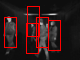
\includegraphics[width=0.9\linewidth]{images/sampleTemplateDetection}
\subcaption{\label{fig:sampleTemplateDetection}}
\end{subfigure}
\begin{subfigure}{0.32\textwidth}
\centering
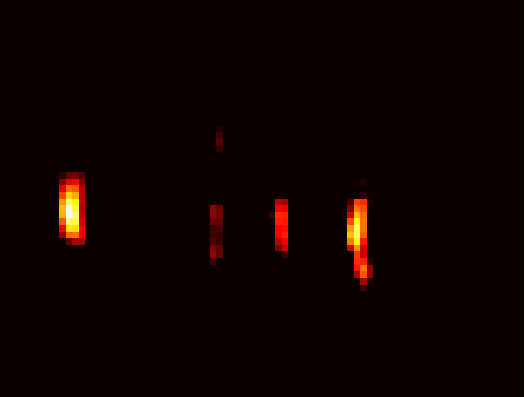
\includegraphics[width=0.9\linewidth]{images/sampleLP}
\subcaption{\label{fig:sampleLP}}
\end{subfigure}

\caption[Poszukiwanie kandydatów za pomocą wzorca probabilistycznego.]{Poszukiwanie kandydatów za pomocą wzorca probabilistycznego. \protect\subref{fig:sampleTemplateDetection} wytypowani kandydaci \protect\subref{fig:sampleLP} mapa LP.}
\end{figure}

Obraz termowizyjny został dopasowany do obrazu wizyjnego, tworząc obraz multispektralny. 
Punkty kalibracyjne zostały wyznaczone na podstawie elementów sylwetek (stopy, dłonie i głowa), od których aktorów wysokość na obrazie wizyjnym wynosiła około 180 pikseli, uzyskując minimum dysparycji między dwoma obrazami dla obiektów poszukiwanych wzorcem o wysokości 30 pikseli. %OK TODO 2 dla mnie to zdanie jest niejasne

Następnie wspołrzędne znalezionych kandydatów podczas badania wzorcem probabilistycznym zostały przeniesione na układ współrzędnych obrazu multispektralnego z~wykorzystaniem parametrów transformacji uzyskanej podczas kalibracji. 
Wokół tych punktów zostały wyznaczone ROI o~wymiarach 80x192 pikseli.
%TODO 2 a można zdanie więcej jak dokładnie... 
Dalej został obliczony wektor cech HOG w każdym z okien, które następnie zostały poddane klasyfikacji za pomocą liniowego SVM.
\begin{figure}[h]
\centering
\begin{subfigure}{0.32\textwidth}
\centering
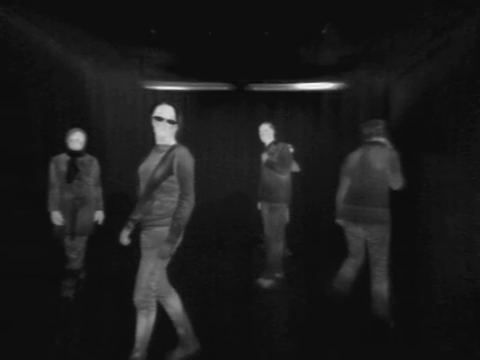
\includegraphics[width=0.9\linewidth]{images/sampleIR}
\subcaption{\label{fig:sampleIR}}
\end{subfigure}
\begin{subfigure}{0.32\textwidth}
\centering
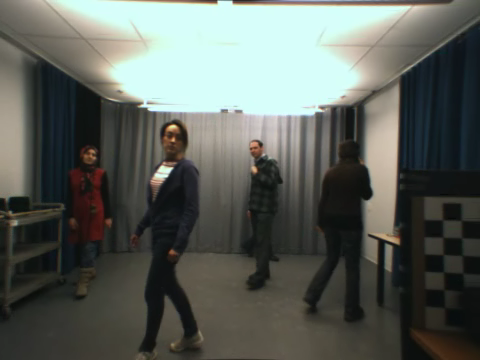
\includegraphics[width=0.9\linewidth]{images/sampleRGB}
\subcaption{\label{fig:sampleRGB}}
\end{subfigure}
\begin{subfigure}{0.32\textwidth}
\centering
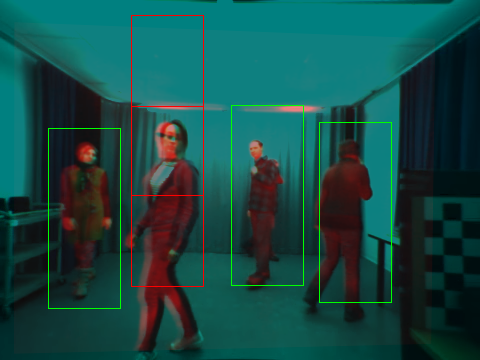
\includegraphics[width=0.9\linewidth]{images/sampleHOGSVM}
\subcaption{\label{fig:sampleHOGSVM}}
\end{subfigure}

\caption[Detekcja]{\protect\subref{fig:sampleIR} Obraz z kamery termowizyjnej, \protect\subref{fig:sampleRGB} obraz z kamery wizyjnej, \protect\subref{fig:sampleHOGSVM} połączone obrazy z zaznaczonymi wynikami detekcji. Zielona ramka oznacza pozytywny wynik klasyfikacji HOG SVM, czerwona -- negatywnie sklasyfikowani kandydaci.}
\end{figure}

Do nauczenia SVM zostały wykorzystane 141 ROI wytypowanych przez wzorzec probabilistyczny. 
Każdemu ROI została przypisana klasa: 1 -- jeżeli zawiera obraz człowieka o~wysokości 160+/-20 px , 0 -- jeżeli jest to element tła bądź część człowieka (np. sama głowa, nogi).

Na 141 próbek 78 stanowiły próbki pozytywne a~62 negatywne. 
SVM sklasyfikował poprawnie pozytywnie 88,9\% próbek zaś poprawnie negatywnie 88,5\%.

%TODO 2 w sumie mało próbek, ale .... trudno

\section{Wykorzystanie AXI-Stream do transmisji sygnału wideo.}

W odróżnieniu od standardowego sposobu przetwarzania strumieniowego wideo, w~AXI4-Stream przesyłane są jedynie aktywne piksele.
Linie synchronizacji poziomej i~pionowej są odrzucane albo przekierowywane do specjalnego bloku, w~którym są mierzone parametry wchodzącego strumienia wizyjnego (liczba pikseli w~linii, liczba aktywnych linii, czas wygaszania itd.).
W~celu wyświetlenia obrazu wykorzystuje się ten sam blok, który ma możliwość generacji nowych sygnałów synchronizacji (ich odtworzenia).

Do transmisji wykorzystane jest 6 sygnałów: dane i~pięć kontrolno-sterujących. 
W~nawiasach są podane linie, które wykorzystuje dany sygnał w~interfejsie AXI4-Stream.
\begin{itemize}
\item \textit{Video Data} (\textit{tdata})-- linia danych o szerokości jednego (albo dwóch) pikseli. Szerokość tej linii powinna być wielokrotnością liczby osiem (16, 24, 48 itd.)
\item \textit{Valid}(\textit{tvalid}) -- linia określająca czy dane piksela są poprawne,
\item \textit{Ready} (\textit{tready})-- linia kontrolna informująca urządzenie master, że \textit{slave} jest gotowy do transmisji danych, 
\item \textit{Start Of Frame} (\textit{tuser}) -- linia sygnalizacyjna pierwszego piksela nowej ramki,
\item \textit{End Of Line} (\textit{tlast})-- linia sygnalizacyjna ostatniego piksela w~linii. 
\end{itemize}

Aby mógł wystąpić poprawny transfer danych linie \textit{Valid} i~\textit{Ready} muszą być w stanie wysokim podczas rosnącego zbocza zegara.
Przykładowe nawiązanie transmisji przedstawia rysunek \ref{fig:handshake}.

\begin{figure}[h]
\centering
\includegraphics[width=1\textwidth]{images/axi-stream_hendshake}
\caption{Przykład rozpoczęcia transmisji Ready/Valid.}
\label{fig:handshake}
\end{figure}


\section{AXI VDMA}
Wiele aplikacji wizyjnych wymaga przechowania całej ramki obrazu w~celu jej dalszej obróbki np. podczas skalowania, przycinania bądź dopasowania liczby klatek na sekundę.
Część programowalna układu Zynq zazwyczaj nie posiada wystarczającej liczby wewnętrznych zasobów pamięciowych do przechowania pełnej klatki obrazu.
Aby stworzyć taki bufor jedną z~możliwości jest wykorzystanie mechanizmu bezpośredniego dostępu do pamięci, który pozwala na przesłanie i~wczytanie danych z logiki programowalnej do pamięci RAM bez konieczności angażowania procesora.
Należy w~tym miejscu zaznaczyć, że dla rozważanej platformy Zybo zewnętrzna pamięć RAM DDR podłączona jest do kontrolera w~systemie procesorowym.

Dostęp ten realizuje się poprzez IP-Core AXI VDMA.
Zapewnia on przejście między interfejsem AXI4-Stream, a~AXI4 Memory Map w~obu kierunkach.
Przed rozpoczęciem przesyłania IP-Core jest konfigurowany poprzez interfejs AXI4-Lite.
Konfiguracja zawiera adres w pamięci RAM do którego ma być zapisana bądź wczytana ramka obrazu.
Po wgraniu do pamięci ramki kontroler może wywołać przerwanie dla systemu procesorowego.

\section{Opis modułów zaimplementowanych w~logice programowalnej}

\subsection{Kontroler kamery IR}
Kamera Lepton przesyła obraz za pomocą interfejsu VoSPI (ang. \textit{Video over Serial Peripheral Interface}). 
W~zastosowanym rozwiązaniu jest on urządzeniem typu \textit{slave}, zaś układ Zynq jest \textit{masterem}. 
Są wykorzystywane 3 z~4 linii typowego kanału SPI: SCK (ang. \textit{Serial Cloack} -- zegar), /CS (ang. \textit{Chip Select} -- wybór układu)(aktywny stanem nikim) oraz MISO (ang. {Master In/Slave Out} – wejście master/wyjście slave).
Transmisja rozpoczyna się od podania stanu niskiego przez kontroler na linii /CS. 
Powoduje to aktywację linii. 
Następnie, \textit{master} rozpoczyna taktowanie zegarem na linii SCK. \textit{Slave} wystawia kolejne bity danych począwszy od MSB (ang. \textit{Most Significant Bit}) na linię MISO. 
Kontroler szczytuje te bity przy każdym rosnącym zboczu zegara do 16 bitowego rejestru przesuwnego.
Dane przesyłane z kamery są zorganizowane w pakiety po 164 bajty. Pakiet rozpoczyna się nagłówkiem składającym się z 2 bajtów pola identyfikacyjnego oraz 2 bajtami sumy CRC. 
Pole identyfikacyjne spełnia dwa zadania. 
Po pierwsze, stanowi 12-bitowy numer pakietu (a~zarazem numer linii obrazu). 
Po drugie, w~przypadku błędnego pakietu zawiera wartość 0xXFXX (X to obojętna wartość) co wskazuje, że nadchodzący pakiet powinien zostać zignorowany przez kontroler. 
Zawartość pakietu stanowi 160 bajtów zawierających wartości 80 pikseli linii. 
W~systemie wykorzystywany jest format RAW14, zatem każdy piksel jest przesyłany w~postaci 2~bajtów zawierających 14 bitową wartość piksela.
Cała ramka obrazu składa się z~63 pakietów. 
60 pierwszych pakietów stanowią linie obrazu zaś ostatnie 3 są przeznaczone na telemetrię, która zawiera m.in. temperaturę matrycy  i~obudowy, 32-bitowy licznik ramek obrazu i bity stanu. %OK TODO 2 FPA Focal plane array z poprzedniego rozdziału??
Pierwsze 3 przesłane pakiety są błędne i~służą do synchronizacji transmisji.
W~przypadku prawidłowego pakietu kontroler szczytuje numer linii obrazu i~wystawia go na wyjściu \textit{row}. 
Następnie na wyjściu \textit{data} wystawiane są wartości kolejnych 80 bitów wraz z~ich pozycją na wyjściu \textit{column}. 
Wysoki stan \textit{we} informuje, że dane są poprawne i~powinny być zapisane.
Wartości \textit{row} i~\textit{column} są zamieniane na adres w~pamięci dwuportowej BRAM, będącą bufor ramki IR. Do zaadresowanej komurki pamięci zapisywana jest wartość piksela z wyjścia \textit{data}. %OK TODO 2 coś zamotane to zdanie...

\subsection {Transformata projekcyjna}

Moduł służy do dopasowania obrazu IR do RGB. 
W~tym celu zamienia współrzędne w~układzie odniesienia obrazu RGB na odpowiadające im w układzie IR. %OK TODO 2 powt. celu
Na wejściu podawany jest strumień AXI4-Stream służący do synchronizacji ramek oraz 12-bitowe współrzędne X i~Y. 
Moduł realizuję operację:
\begin{equation}
\begin{bmatrix}
u_n & v_n & n
\end{bmatrix}
=
\begin{bmatrix}
x & y & 1
\end{bmatrix}
T
\end{equation}

\begin{equation}
u = \frac{u_n}{n}
\end{equation}

\begin{equation}
v = \frac{v_n}{n}
\end{equation}

\noindent
gdzie $x$, $y$ to współrzędne obrazu w~układzie odniesienia kamery wizyjnej, $u$, $v$ to odpowiadające im współrzędne w~układzie odniesienia kamery termowizyjnej. 
$T$ to macierz transformacji.

Moduł wystawia na wyjściu strumień wizyjny AXI4-Stream, 12-bitowe wartości U i V oraz ich części ułamkowe w~U\_fraction i~V\_fraction (14 bitów). 
W~module zostały wykorzystane 34 z~80 dostępnych w~układzie Zynq (wersji na karcie Zybo) modułów DSP48 do wykonania operacji arytmetycznych, z~czego większość wychodzi w~skład IP-Core dzielarki dostarczonej przez producenta układu (14 na pojedyńczą dzielarkę).
%% Do implementacji jednej dzielarki zostało wykorzystane 14 modułów DSP. %TODO OK powt. to jakoś trzeba złączyć z poprzednim
Dzielenie nie odbywa się w~pełni potokowo. 
Użyty w dzielarce algorytm \textit{High\_Radix} wymaga zatrzymania strumienia na czas obliczeń. 
Zmniejszenie liczby instancji dzielarek pozwoliło na zaoszczędzenie pewnej liczby (jak się później okazało istotnej) zasobów logicznych.
Jednak dzięki zastosowaniu wyższej częstotliwości niż zegar pikseli obrazu RGB oraz bufora (250 MHz) nie stanowi to wąskiego gardła systemu. 
Macierz transformacji T jest zapisana w~dziewięciu 32-bitowych rejestrach i~konfigurowalna poprzez interfejs AXI4-Lite.
Elementy macierzy są 25 liczbami w notacji stałoprzecinkowej: 1 bit znaku 10 -- część całkowita, 14 -- część ułamkowa. 
Taka dokładność pozwala na maksymalne wykorzystanie pojedynczych modułów DSP48 (gdyż wejście B jest 25-bitowe). 
Rysunek \ref{fig:transfProjek} przedstawia schemat modułu.
\begin{figure}
\centering
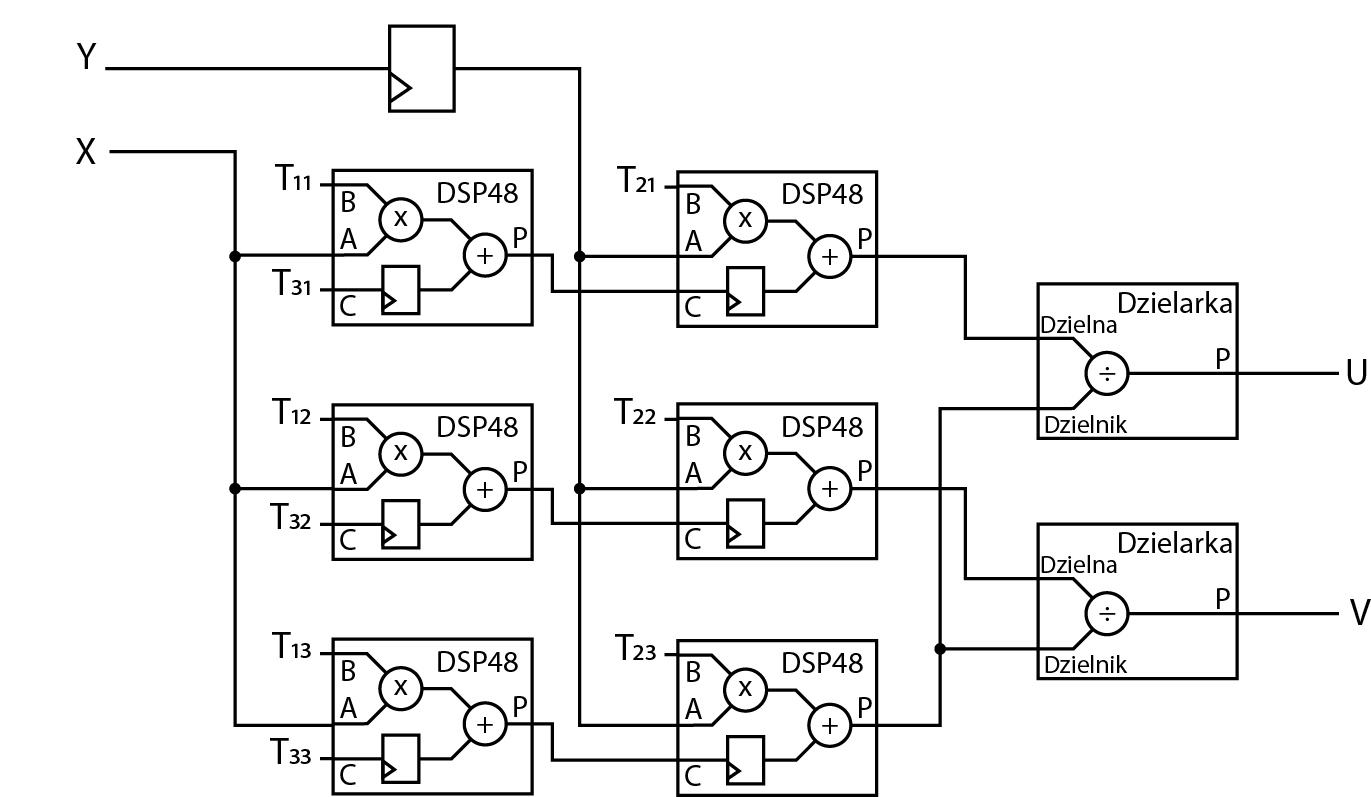
\includegraphics[width=0.70\linewidth]{images/transfProjek.png}
\caption[Schemat modułu transformacji projekcyjnej.]{Schemat modułu transformacji projekcyjnej.}
\label{fig:transfProjek}
\end{figure}

\subsection{Interpolacja dwuliniowa} 
%% Ma za zadanie pobrać z pamięci dwuportowej obrazu IR wartość piksela wskazaną na wejściu układu i wystawić na wyjście. %TODO OK??? a coś jeszzce zrobić -- bo to jest kontorler....
Moduł pozwala na interpolację wartości piksela wskazanego przez koordynaty na wejściu.
Podobnie jak reszta systemu używa AXI4-Stream do przekazywania danych między poszczególnymi modułami.
Dane na wejściu to współrzędne U i~V oraz ich części ułamkowe U\_fraction ($U_f$) i~V\_fraction ($V_f$).
Moduł został wyposażony w~4 rejestry, w~których przechowywane są współrzędne oraz wartości 4 ostatnio użytych pikseli.
Zabieg ten znacznie redukuje liczbę potrzebnych zapytań do pamięci.
Podczas powiększania obrazów istnieje duża szansa, że kolejne koordynaty na wejściu U, V odwołają się do tych samych czterech otaczających ich pikseli (np. [0,0], [1,0], [2,0], podczas zwiększania 10-krotnego, wynikiem transformacji byłyby punkty: [0,0], [0.1,0], [0.2,0], ... więc w~celu interpolacji odwoływałyby się do wartości otaczających ich pikseli: [0,0] , [1,0], [0,1], [1,1]).
W~module następuje sprawdzenie, czy w~pamięci są już wartości z~koordynatów [U, V], [U+1, V] [U, V+1], [U+1, V+1].
Jeżeli któregoś piksela brakuje, jest on pobierany z pamięci i~zapisywany w rejestrze przechowującym niepotrzebny piksel.
Jeżeli wszystkie koordynaty się zgadzają, obliczana jest wartość piksela wyjściowego zgodnie ze wzorem \eqref{equ:bilinear}.

\begin{equation}\label{equ:bilinear}
Ir = A(1-U_{f})(1-V_{f})+B(1-V_{f})+C(1- U_{f})V_{f}+ D U_{f} V_{f}
\end{equation}
\noindent gdzie: $ A, B, C,D $ odpowiadają wartościom pikseli w [U, V], [U+1, V] [U, V+1], [U+1, V+1], a $ Ir $ to wartość wyjściowa piksela wyjściowego.

Moduł działa potokowo. 
W~przypadku gdy wymagana jest  aktualizacja rejestrów, strumień jest wstrzymywany na czas pobrania stosownych wartości z~bufora ramki IR.
Jeżeli koordynaty wejściowe wychodzą poza zakres obrazu termowizyjnego, to ich wartość wyjściowa odgórnie wynosi zero.

\subsection{Łączenie strumieni}

Moduł posiada dwa wejścia AXI4-Stream. 
Strumień RGB jest nadrzędny i~do niego jest dołączany strumień IR. Do synchronizacji została wykorzystana możliwość wstrzymania transmisji poprzez linię \textit{tready} w~interfejsie AXI4-Stream.
Piksele z~dołączanego obrazu są odrzucane do momentu pojawienia się sygnału SOF, reprezentowanym przez wysoki stan linii \textit{tuser}.
Następnie, w~momencie pojawienia się sygnału SOF w~strumieniu głównym transmisja zostaje ponownie wznowiona. 
Po przejściu całej ramki strumienie są ponownie synchronizowane.

\subsection{Koloryzacja i nakładanie}

Strumień RGBIR zostaje połączony w~jeden obraz.
Obraz IR zostaje poddany koloryzacji na podstawie wartości zapisanych w~12-bitowym LUT (ang. \textit{Lookup table}). 
Rysunek \ref{fig:jetPalet} przedstawia użytą paletę do wizualizacji temperatury. 
Obrazy nakładają się w proporcjach 50 na 50. 
Jeżeli wartość piksela IR jest równa zero to nie jest on wyświetlany.
Na wyjściu jest podany 24-bitowy strumień RGB. 
Przykładowy wynik operacji przedstawiono na rysunku \ref{fig:koloryzacja}.
\begin{figure}
\centering
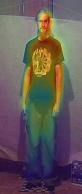
\includegraphics[width=0.3\linewidth]{images/koloryzacja.jpg}
\caption[Obraz IR po koloryzacji i nakłądaniu.]{Obraz IR po koloryzacji i nakładaniu.}
\label{fig:koloryzacja}
\end{figure}

\begin{figure}
\centering
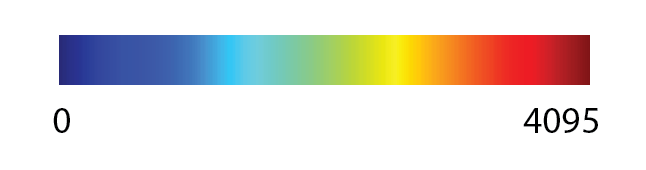
\includegraphics[width=0.5\linewidth]{images/jetPalet.png}
\caption[Paleta kolorów użyta do wizualizacji temperatury.]{Paleta kolorów użyta do wizualizacji temperatury.}
\label{fig:jetPalet}
\end{figure}

\subsection{Obramowanie wyników}

Moduł ma na celu wskazanie na obrazie lokalizacji wykrytego przechodnia, poprzez obramowanie tego obszaru ramką określonego koloru. Kolor, rozmiar i~lokalizacja ramki jest zapisana w dwóch 32-bitowych rejestrach, konfigurowalnych poprzez interfejs AXI4-Lite.

\subsection{Moduł DPM}

Moduł został zaczerpnięty z pracy inżynierskiej autora w~celu selekcji kandydatów w~obrazie multispektralnym i~jest opisany w rozdziale \ref {sec:xiao_2015}. 
Do detekcji wykorzystuje bezpośredni strumień pikseli kamery termowizyjnej. 
Pomocniczy moduł \textit{data grabber} znajdujący się tuż za kontrolerem kamery IR ma za zadanie rozdzielenie sygnału do dwóch komponentów: bufora ramki oraz, po zbinaryzowaniu, do modułu DPM wraz z~jego koordynatami. 
Moduł składa się z~okna kontekstowego o~wymiarach 16x40 pikseli, gdzie odbywa się porównanie z macierzą wzorcową. 
Do każdego piksela w~oknie przypisywana jest wartość ze wzorca LPBW -- jeżeli piksel jest biały albo LPMB w~przypadku czarnego. 
Następnie, wszystkie wartości są sumowane za pomocą drzewa sumacyjnego. Wynikiem jest wartość wyjściowa LP (ang. \textit{Logarithmic Probability}). 
Jeżeli przekroczy ona wartość progową (ustaloną na podstawie sumy LP policzoną dla tła i~parametru K) zostaje przesłana do listy kandydatów wraz ze współrzędnymi tego okna (w~układzie odniesienia kamery IR).
Lista kandydatów jest na bieżąco przesyłana za pomocą AXI4-Stream do pamięci systemu procesorowego poprzez AXI DMA. 
Po sprawdzeniu ostatniego okna zostaje przesłany sygnał \textit{tlast} i~moduł AXI DMA wygeneruje przerwanie w~systemie procesorowym. 
Wartość progowa binaryzacji i~LP jest konfigurowalna za pomocą AXI4-Lite.

\section{System procesorowy}

Program działający w~części procesorowej układu Zynq spełnia dwa podstawowe zadania. 
Po pierwsze pozwala na konfigurację modułów znajdujących się w~PL za pomocą AXI4-Lite. 
Użytkownik za pośrednictwem konsoli może wprowadzać własne parametry dla każdego z modułów. 
Program pozawala również na zapis na karcie SD pojedynczej klatki obrazu multispektralnego, następnego wykrytego ROI oraz ROI znajdującego się pośrodku sceny. 
Ta opcja ułatwiła tworzenie bazy do nauczenia klasyfikatora SVM.

Drugim zadaniem jest klasyfikacja wytypowanego przez DPM kandydata. 
Po otrzymaniu przerwania przez moduł AXI DMA powiązany z DPM, sprawdzana jest lista kandydatów i wybierany jest ten o~największej wartości LP. 
Współrzędne kandydata są podane w~układzie odniesienia kamery IR. 
Po przeliczaniu ich za pomocą macierzy transformacji projekcyjnej i~dodaniu pewnego \textit{offsetu} w~buforze ramki obrazu RGBIR zostaje wskazane ROI o~wymiarach 80x192 pikseli. 
Następnie, obliczany jest wektor cech HOG z~tego obszaru. 
Potem na jego podstawie odbywa się klasyfikacja przy użyciu wytrenowanego SVM. 
Wynik klasyfikacji jest wyświetlany w~konsoli wraz z~jego współrzędnymi na obrazie i~wartością LP. 
Dodatkowo obszar ten zostanie zaznaczony zieloną ramką na wyjściowym strumieniu wizyjnym. 
Jeżeli kandydat nie zostanie zakwalifikowany pozytywnie przez SVM ramka przybierze kolor czerwony. 
Brak kandydatów wskazuje czarna ramka w~miejscu ostatniej detekcji.

\section{Proces kalibracji}
W~celu kalibracji, zostaje wykonane zdjęcie specjalnej planszy kalibracyjnej za pomocą obu kamer (rysunki \ref{fig:calibrationThermal}, \ref{fig:calibrationRGB}). 
%OK TODO 2 a co to ,,świeci'' na tej planszy...
Pozwala to na identyfikację czterech punktów kalibracyjnych w~obu przestrzeniach: RGB i~IR. W użytej planszy zastosowano rozgrzane kawałki metalu jako punkty odniesienia.
Następnie na ich podstawie zostaje obliczona macierz transformacji projekcyjnej. 
Na rysunku \ref{fig:calibrationCorrectedGrey} przedstawiono obraz z~kamery termowizyjnej po transformacji, który pokrywa się z obrazem wizyjnym (rysunek \ref{fig:calibrationSum}).

\begin{figure}[h]
\centering
\begin{subfigure}{0.47\textwidth}
\centering
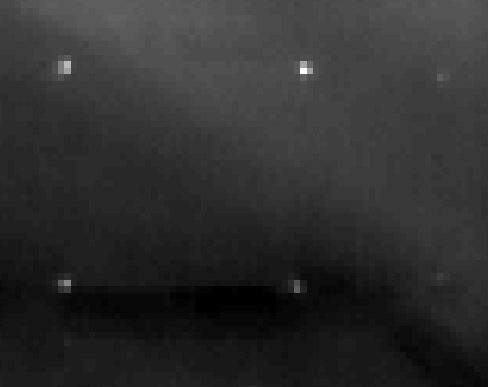
\includegraphics[width=0.9\linewidth]{images/calibrationThermal}
\subcaption{\label{fig:calibrationThermal}}
\end{subfigure}
\begin{subfigure}{0.47\textwidth}
\centering
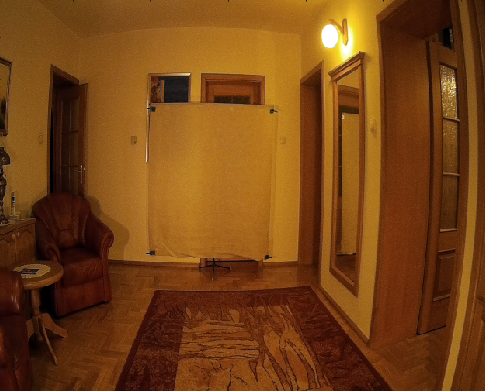
\includegraphics[width=0.9\linewidth]{images/calibrationRGB}
\subcaption{\label{fig:calibrationRGB}}
\end{subfigure}
\begin{subfigure}{0.47\textwidth}
\centering
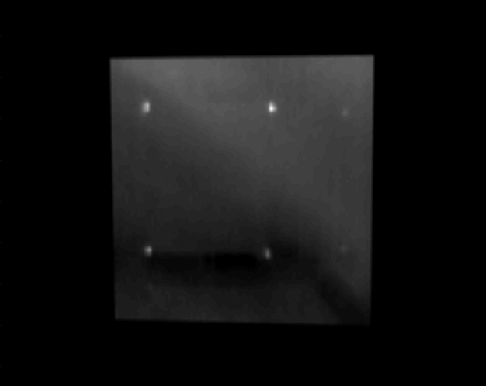
\includegraphics[width=0.9\linewidth]{images/calibrationCorrectedGrey}
\subcaption{\label{fig:calibrationCorrectedGrey}}
\end{subfigure}
\begin{subfigure}{0.47\textwidth}
\centering
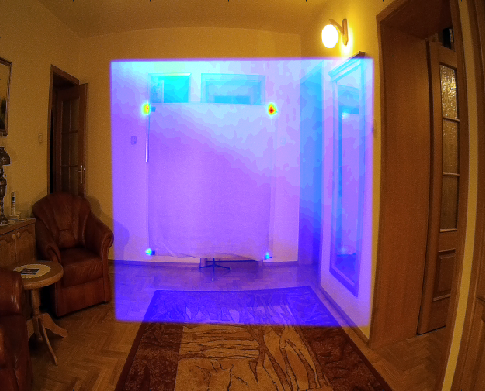
\includegraphics[width=0.9\linewidth]{images/calibrationSum}
\subcaption{\label{fig:calibrationSum}}
\end{subfigure}
\caption[Proces kalibracji]{Proces kalibracji: \protect\subref{fig:calibrationThermal} obraz z kamery termowizyjnej, \protect\subref{fig:calibrationRGB} obraz z kamery wizyjnej, \protect
\subref{fig:calibrationCorrectedGrey} obraz z kamery termowizyjnej po transformacji projekcyjnej, \protect\subref{fig:calibrationSum} obraz z kamery termowizyjnej po transformacji projekcyjnej nałożony na obraz z kamery wiyjnej.}
\end{figure}

\section{HOG i SVM}
W pierwszym etapie tworzony jest wektor cech HOG. Dla każdego piksela w ROI zostaje obliczony gradient składający się z kierunku oraz modułu.
Następnie okno detekcji zostaje podzielone na 60 komórek o wielkości 16x16 pikseli. 

%OK TODO 2 coś nie halo 1. Gradienty. 2. Potem podział.
%TODO 2 jakieś zdanie wprowadzenia ?

%TODO Gradient dla pojedynczego piskela ma amplitude (moduł) i kierunek.

%TODO Teraz podział i obliczanie histogramu w komórkach

Dla każdej z komórek zostaje obliczony histogram ważony o 9 przedziałach. 

Oznacza to, że wartość moduł gradientu jest dzielona na dwa przedziały, pomiędzy którymi się znajduje w proporcjach określonych wzorem \eqref{equ:bin1}, \eqref{equ:bin2}.
%TODO wypadkowa -> moduł !!
\begin{equation}\label{equ:bin0}
Bin1_{dir} < G_{dir} < Bin2_{dir}
\end{equation}
\begin{equation}\label{equ:bin1}
Bin1_{mag} = \frac{Bin2_{dir} - G_{dir}}{Bin2_{dir} - Bin1_{dir}}
\end{equation}
\begin{equation}\label{equ:bin2}
Bin2_{mag} = \frac{G_{dir}- Bin1_{dri}}{Bin2_{dir} - Bin1_{dir}}
\end{equation}
\noindent gdzie: $G_{dir}$ to kierunek badanego gradient, $G_{mag}$ to wypadkowa badanego gradientu, $Bin1_{dir}$,$Bin2_{dir}$ to kierunki gradientów powiązane z danym przedziałem histogramu, $Bin1_{mag}$,$Bin2_{mag}$ to wypadkowe gradientu przypisana do poszczególnego z przedziału.
%ok TODO wypadkowe.... 

Dla każdej z komórek dodatkowo obliczana jest suma kwadratów wartości przedziałów histogramu.
Następnie komórki są łączone w~bloki 2 na 2, w~których obrębie dokonywana jest normalizacja, wykorzystując wcześniej obliczone sumy kwadratów. 
Zastosowano normalizację L2 wyrażoną wzorem \eqref{eq:norm}.
\begin{equation}\label{eq:norm}
norm = \sqrt{\sum_{i} (Bin(i)_{mag})^2 + c}
\end{equation}
\noindent gdzie: $Bin(i)_{mag}$ to wartość przedziału histogramu, a $c$ to mała wartość stała.
Następnie wartości wszystkich 36 przedziałów w~4 histogramach są dzielone przez $norm$.
Bloki nakładają się na siebie, zatem w~pojedynczym oknie można wyodrębnić 44 bloki. 
Suma histogramów z~wszystkich bloków tworzy 1584-elementowy wektor cech.


%OK TODO 2 a to zdanie do czego... nie pasuje kompletnie... i nieco szerszy opis SVM.
Maszyna wektorów nośnych jest modelem służącym do określanie przynależności wektora cech do jednej z klas. W procesie nauczania tworzona jest superpłaszczyzna oddzielająca przykładowe próbki tych dwóch klasy z największym możliwym marginesem między nimi. Próbki znajdujące się na marginesie nazywane są wektorami nośnymi. W~celu wytrenowania klasyfikatora zostało wykonane 60 obrazów -- 30 pozytywnych zawierających przechodnia i~30 przedstawiają elementy tła lub niekompletnej sylwetki człowieka (np. sama ręka). Po nauczeniu do każdego elementu wektora cech przypisana jest jego waga oraz wartość progowa -- $bias$.
Wynik sumy iloczynów wag i cech wektora oraz $biasu$ stanowi podstawę do klasyfikacji. Jeżeli jest większy od zera świadczy to o~pozytywnym wyniku klasyfikacji.

%OK TODO iloczyn wagi i cechy jak już. 

\section{Wyniki}

Aby sprawdzić działanie i~dokładność systemu została zaimplementowana możliwość zapisu obliczonego wektora cech na karcie SD.
Następnie został obliczony przykładowy błąd względny między wektorem cech wyliczonym w pakiecie Matlab, a uzyskanym z systemu wizyjnego. %TODO 2 powt. obliczony i dlaczego przykładowy ?
Błąd oscyluje w~granicy \(10^{-6}\) co czyni go marginalnym i~najprawdopodobniej wynika z~różnic w użytych bibliotekach numerycznych. 
Świadczy to o prawidłowym działaniu systemu.

Na przebadanie jednego okna zaproponowany system potrzebuje 75 ms (dla porównania te same obliczenia w~pakiecie Matlab zajmują około 23 ms przy użyciu komputera z procesorem Pentium Core i7 i~8GB pamięci RAM).
Dzięki zastosowaniu sprzętowego wyszukiwania ROI zadanie systemu procesorowego zostało ograniczone do analizy pojedynczego ROI. 
Kamera termowizyjna, będąca źródłem sygnału dla wzorca probabilistycznego, pracuje z prędkością 9 klatek na sekundę co zapewnia 111 ms na analizę jednej rami obrazu. 
Ponieważ analiza jednego okna zajmuje 75 ms  możliwe sprawdzenie tylko jednego ROI na ramkę. 
Na rysunku \ref{fig:workingSystem} przedstawiono zdjęcie działającego systemu.

\begin{figure}
\centering
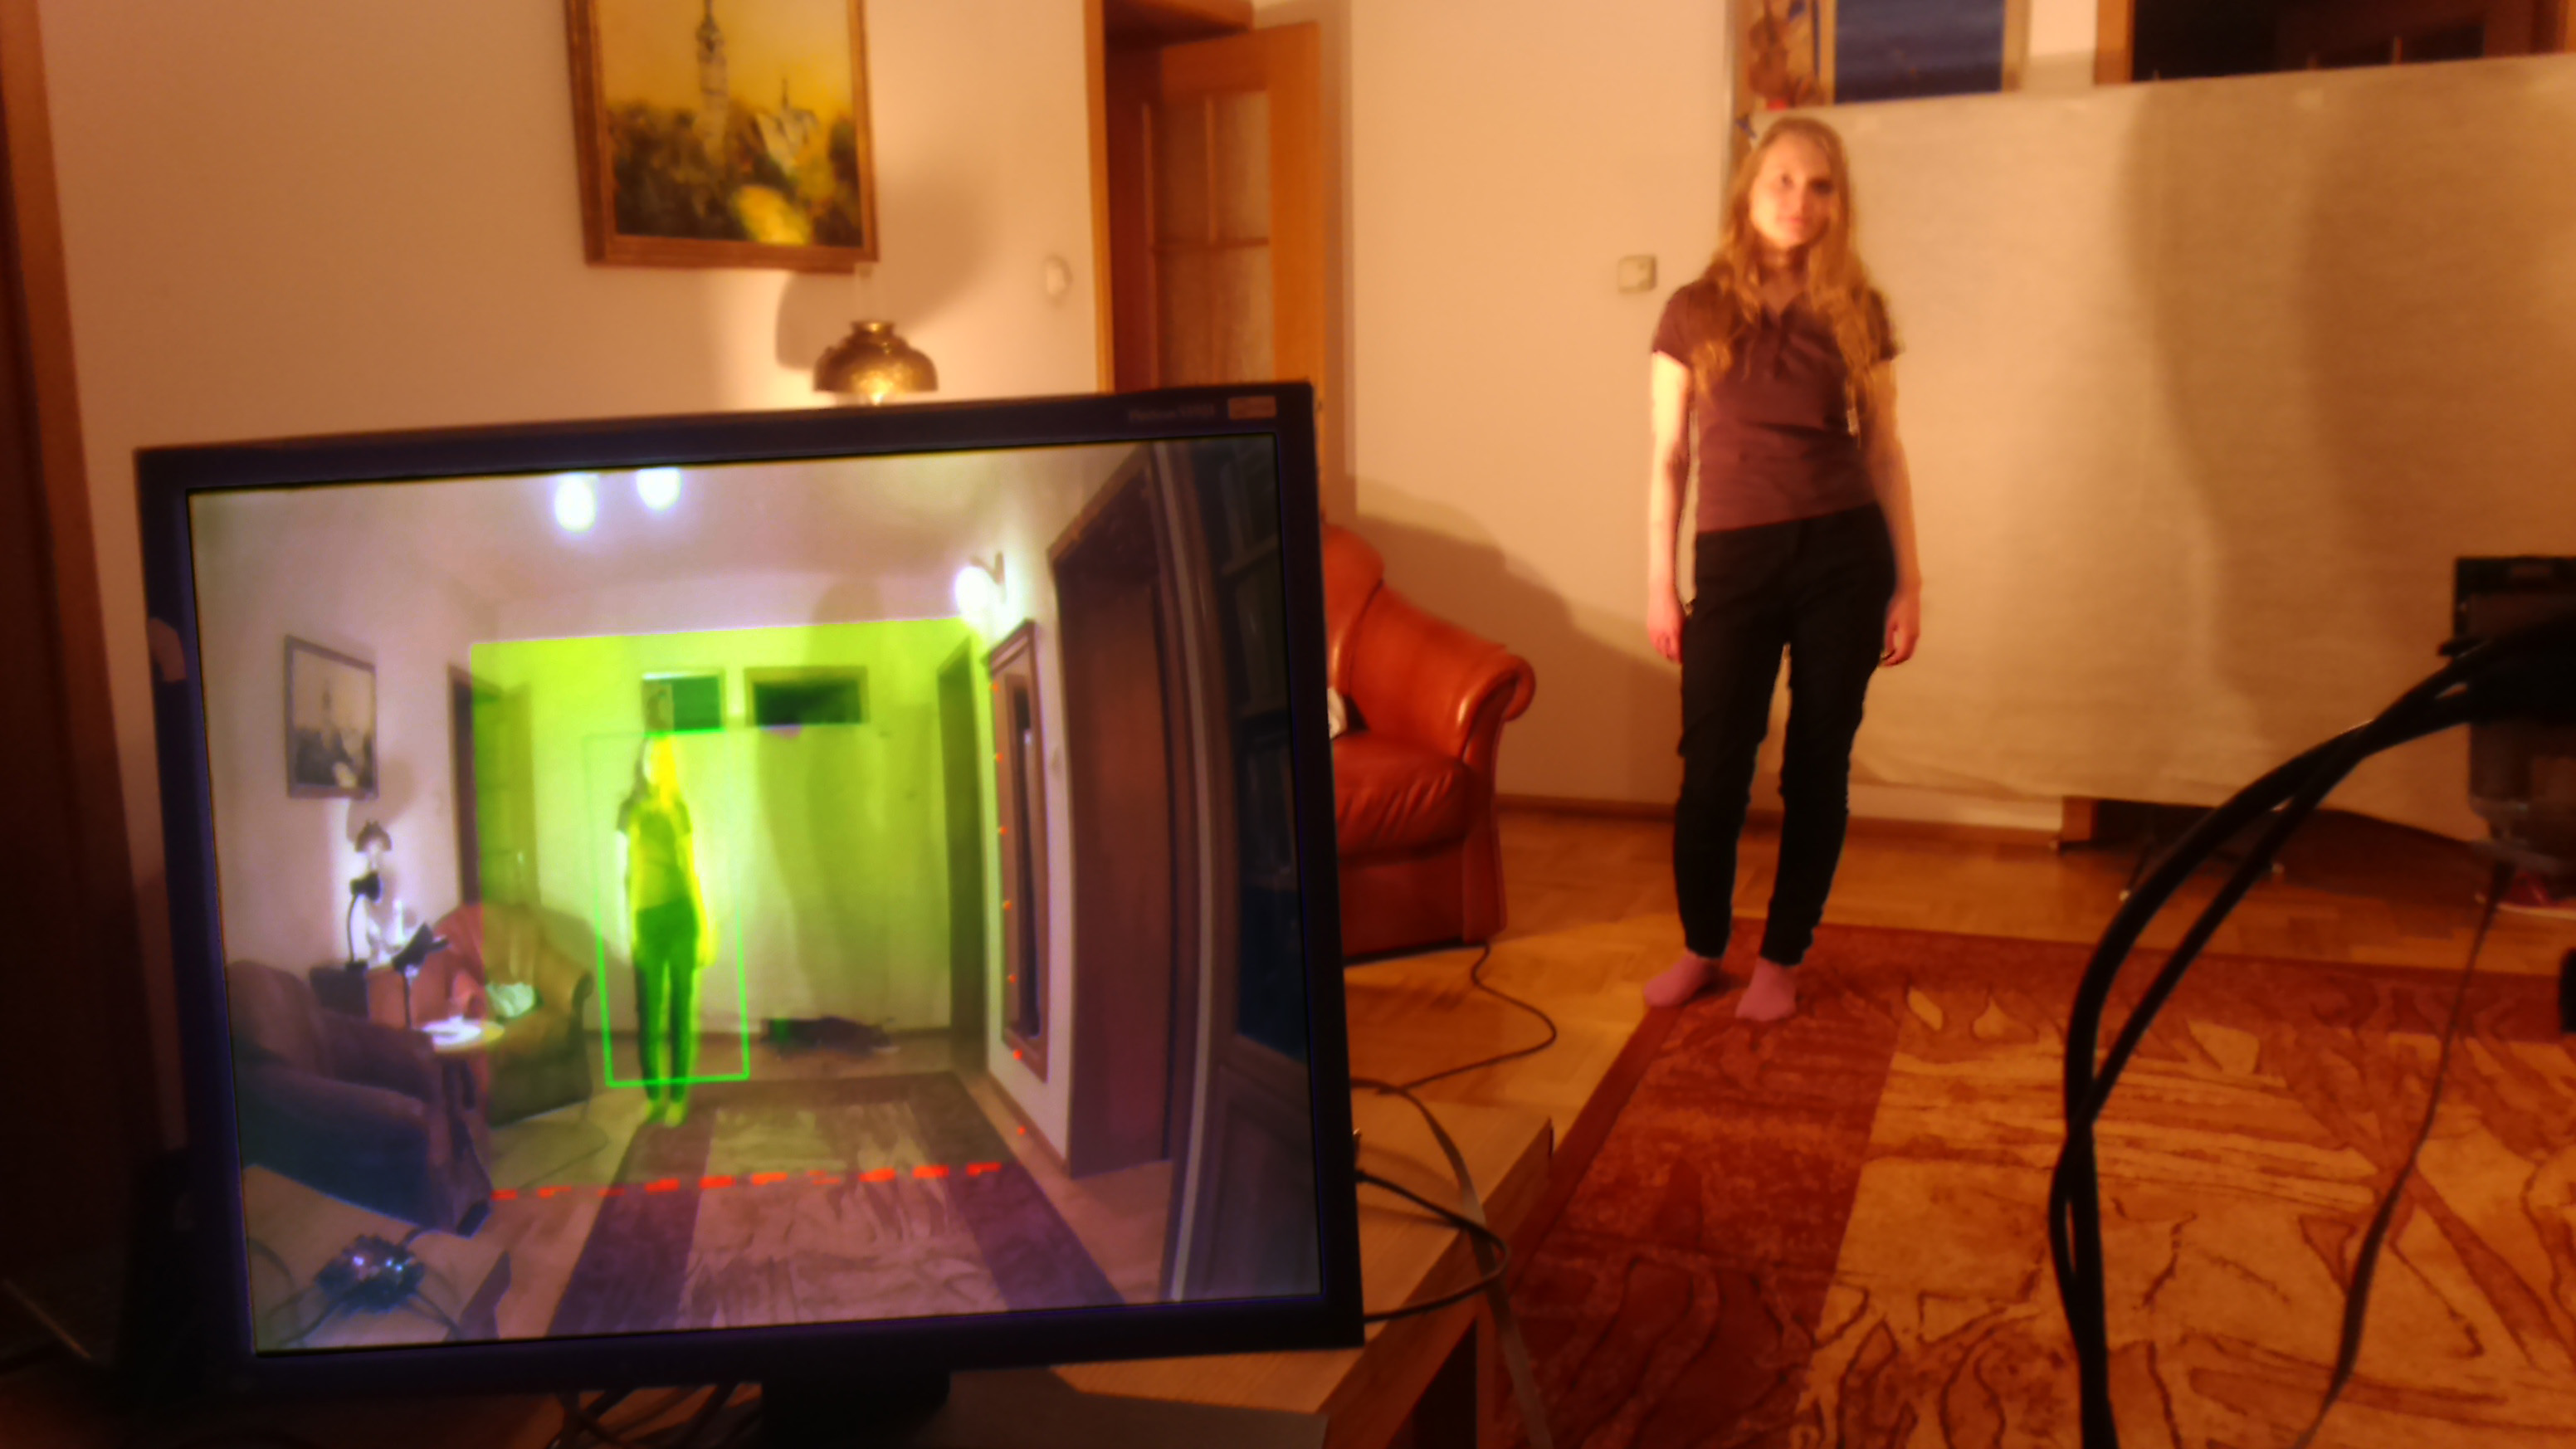
\includegraphics[width=0.8\linewidth]{images/workingSystem.jpg}
\caption[Działający system.]{Działający system.}
\label{fig:workingSystem}
\end{figure}

%TODO no ale jakby to dla 30/60 fps... to już tak pięknie nie jest %% TT Mam w zapasie moduł który liczy gradienty oraz przedział i histogram pojedynczego piksela, tylko dodanie go powoduje że układ jest niesyntezowalny
%OK TODO 2 to to w future work...
W~tabeli \ref{tab:fpgautilization} zostało przedstawione wykorzystanie zasobów logiki programowalnej. Najwięcej zasobów LUT zostało wykorzystane w module DPM. Spowodowane jest to implementacją  dużego okna kontekstowego wraz z drzewem sumacyjnym. Z kolei większość modułów DSP48 została wykorzystana do dzielarek w module transformaty projekcyjnej, gdzie odbywa się najwięcej obliczeń arytmetycznych.
\begin{table}[]
\centering
\caption{Wykorzystane zasoby logiki programowalnej.}
\label{tab:fpgautilization}
\begin{tabular}{|l|l|l|l|}
\hline
Element & Wykorzystane & Dostępne & \% \\ \hline 
LUT & 12583 & 17600 & 71,49 \\ \hline
LUTRAM & 617 & 6000 & 10,28 \\ \hline
FF & 19924 & 35200 & 56,60 \\ \hline
BRAM & 25,50 & 60 & 42,50 \\ \hline
DSP & 36 & 80 & 45,00 \\ \hline
IO & 43 & 100 & 43,00 \\ \hline
BUFG & 7 & 32 & 21,88 \\ \hline
MMCM & 1 & 2 & 50,00 \\ \hline
PLL & 1 & 2 & 50,00 \\ \hline
\end{tabular}
\end{table}



%OK TODO 2 Tu mogłby Pan kilka zdań komentarza do tabelki. Co jest przyczyną takiego, a nie innego wykorzystania.
